\section{格点矩阵元与模拟设置}\label{sec:setup}

格点矩阵元标准的非微扰重正化方法是：计算该算符的一些辅助矩阵元（它们也可以在微扰论中计算），并用它们作为重正化因子来趋近连续极限。本文聚焦于研究可能对准光前关联的重正化有用的辅助矩阵元。我们主要考虑以下几种情形下准 PDF 算符的矩阵元：1）大欧氏动量的夸克态中；2）强子（如 $\pi$ 或核子）的物理零动量态中。我们还将研究真空中的矩阵元~\cite{Braun:2018brg}（情形 3），并由算符乘积展开（OPE）可以表明：由于小 $z$ 时这种矩阵元被压低，它并不是好的重正化选择。此外，由于依赖 $z$ 的重正化主要与 Wilson 链接相联系，我们也将考虑 Wilson 圈以及固定规范下 Wilson 链接的矩阵元（情形 4）。

我们在静止系中计算 $\pi$ 与核子矩阵元 $\tilde{h}^{0}_{H}(z)=\langle H| O_{\gamma_t}(z)|H \rangle_{\vec{P}=0}$，即计算如下三点关联函数，
\begin{align}\label{eq:hadron}
&R_{H}(t_2,t,z)\equiv\frac{\langle O_H(t_2)\sum_{\vec{x}}O_{\gamma_t}(z;(\vec{x},t))O_H^{\dagger}(0)\rangle}{\langle O_H(t_2)O_H^{\dagger}(0)\rangle}\nonumber\\
&=\langle H| O_{\gamma_t}(z)|H \rangle\nonumber\\
&+{\cal O}(e^{-\delta m t})+{\cal O}(e^{-\delta m (t_2-t)})+{\cal O}(e^{-\delta m t_2}),
\end{align}
其中 $O_{\gamma_t}(z,(\vec{x},t))=\bar{\psi}(\vec{x},t) \gamma_t U((\vec{x},t),(\vec{x}+\hat{n}_z z,t)) \psi (\vec{x}+\hat{n}_z z,t)$，$\hat{n}_z$ 是沿 $z$ 方向的单位矢量，$O_H$ 是诸如 $\pi$ 或核子等强子的插值场；$t_2$ 对应源--汇分离。

为了精确地得到 $\tilde{h}^0_{H}(z)$，需要 $t$ 与 $t_2-t$ 都足够大以压制激发态污染，或者用恰当的参数化拟合三点函数以处理激发态污染。对 $\pi$ 情形可以采用第一种策略，因为静止系中 $\pi$ 的信噪比不会衰减；而对统计误差随 $t$ 与 $t_2$ 指数增长的其他情形，第二种策略必不可少。受（反）周期边界条件限制，$t_2$ 至多取 $T/2$，在现代大多数格点系综中它大于 2 fm。由于 $\pi$ 基态与第一激发态之间的质量劈裂 $\delta m\sim $ 1 GeV，$\langle \tilde{h}^0_{\pi}(z)\rangle$ 能够以足够的精度提取出来。在小微扰 $z$ 处，$\langle \tilde{h}^0_{\pi}(z)\rangle^{-1}$ 在一定的 ${\cal O}(\Lambda_{\rm QCD}^2z^2)$ 幂次修正范围内充当重正化因子~\cite{Orginos:2017kos}。

含定域算符的格点 QCD 矩阵元常用的非微扰重正化方法是 RI/MOM 方案~\cite{Martinelli:1994ty} 及其修正版本~\cite{Aoki:2007xm}：在给定动量的离壳夸克态中分别于格点与维数正规化下计算裸矩阵元，然后在 $\overline{\textrm{MS}}$ 方案下重正化二者的差，从而得到裸量的重正化因子。对准 PDF 而言，这样的重正化常数（RI/MOM 重正化因子）由给定动量 $p^2$ 的离壳夸克态中的 $O_{\gamma_t}(z)$ 矩阵元定义为~\cite{Green:2017xeu,Chen:2017mzz,Alexandrou:2017huk,Stewart:2017tvs}
\begin{align}\label{eq:Z_ri}
&Z^{RI}(z,\mu_R)=\frac{1}{4N_c}\textrm{Tr}[\gamma_t\langle q|O_{\gamma^t}(z)|q\rangle]|_{p^2=-\mu_R^2,p_z=p_t=0},
\end{align}
其中 $N_c=3$ 是色数，$\mu_R$ 是 RI/MOM 重正化标度。我们取 $\mu_R$ = 3 GeV，因为 RI/MOM 因子在某一范围内对标度依赖很小~\cite{Zhang:2020rsx}。我们在 Landau 规范固定的组态上进行计算，并选取 $p_z=p_t=0$ 以消除不同投影之间的差别~\cite{Liu:2018uuj}。

因子 $Z^{RI}$ 可以对任意格点正规化——等价地说，对格点上定义的任何夸克与规范作用量——作非微扰计算。然而，目前的格点 QCD 计算限于 Landau 规范，Landau 规范下离壳态的微扰匹配在一圈以上可能相当复杂~\cite{Chen:2020ody}。

重正化中依赖 $z$ 的部分来自 Wilson 线，因此可以从纯 Wilson 线的矩阵元中提取线性发散。首先可以考虑 Wilson 圈~\cite{Chen:2016fxx,Zhang:2017bzy,Musch:2010ka,Green:2017xeu,Chen:2017gck},
\begin{equation}
{\cal U}(r,t)=\langle U(\vec{r},t;\vec{r},0)U(\vec{r},0;\vec{0},0)U(\vec{0},0;\vec{0},t)U(\vec{0},t;\vec{r},t)\rangle ,
\end{equation}
文献~\cite{Chen:2016fxx} 提出用这一方案重正化 $\pi$ DA，并在随后的 K 介子 DA 研究~\cite{Zhang:2017bzy} 中基于多个格点间距的计算精确提取了线性发散系数。但此后大多数格点 QCD 计算转而采用 RI/MOM 方案或强子矩阵元。

也可以考虑单个 Wilson 链接在固定规范（如 Landau 规范）下的矩阵元 $\langle U(0,z)\rangle$。作为不带任何外部态的最简单选择，$\langle U(0,z)\rangle$ 可以提供一种参照，用以判别线性发散行为是否对外部态的存在敏感，正如准 PDF 算符可乘重正化性研究所建议的那样~\cite{Ji:2015jwa, Ji:2017oey,Ishikawa:2017faj,Green:2017xeu}。

\begin{table}[htbp]
  \centering
  \begin{tabular}{c|ccrc}
  \toprule
 符号 & $6/g^2$ & $L$ & $T$  & $a(\mathrm{fm})$ \\
\hline
a12m310 &  3.60 & 24 & 64  & 0.1213(9) \\
\hline
a09m310 &  3.78 & 32 & 96 & 0.0882(8)  \\
\hline
a06m310 &  4.03 & 48 & 144 & 0.0574(5) \\
\hline
a04m310 &  4.20 & 64 & 192 & 0.0425(4)  \\
\hline
a03m310 &  4.37 & 96 & 288 & 0.0318(3) \\
\hline
  \end{tabular}
  \caption{MILC 系综的设置，包括裸耦合常数 $g$、格点大小 $L^3\times T$ 与格点间距 $a$。}
  \label{tab:lattice}
\end{table}

\begin{table}[htbp]
  \centering
  \begin{tabular}{c|ccrccc}
  \toprule
 符号 & $6/g^2$ & $L$ & $T$ &  $a(\mathrm{fm})$\\
\hline
DW11 & 2.13 &24 & 64  & 0.1105(3) \\
\hline
DW08 & 2.25 &32 & 64  & 0.0828(3) \\
\hline
DW06 & 2.37 &32 & 64  & 0.0627(3) \\
\hline
  \end{tabular}
  \caption{RBC 系综的设置，包括裸耦合常数 $g$、格点大小 $L^3\times T$ 与格点间距 $a$。}
  \label{tab:lattice2}
\end{table}

我们的格点计算使用 Chroma 软件套件~\cite{Edwards:2004sx}、QUDA~\cite{Clark:2009wm,Babich:2011np,Clark:2016rdz} 以及 HIP 编程模型~\cite{Bi:2020wpt}。我们使用 MILC 合作组~\cite{Bazavov:2012xda} 生成的五档格点间距、$2+1+1$ 味（简并的上/下夸克、奇异与粲自由度）高度改进交错夸克（HISQ）组态，以及 RBC/UKQCD 合作组~\cite{Blum:2014tka} 生成的三档格点间距、$2+1$ 味畴壁（DW）夸克加 Iwasaki 规范组态。所有系综都依据相应系综中海夸克质量对应的 $\pi$ 质量，把 $\pi$ 质量调到约 310 MeV。MILC 系综的格点间距依据文献~\cite{Miller:2020evg} 确定的参数由 Wilson 流测定。

我们使用不经超立方（HYP）涂抹的矩阵元来检验微扰重正化的分析（第~\ref{sec:test}、\ref{sec:StrtoRe} 和~\ref{sec:highorder} 节）。然而，实际计算中不涂抹的结果可能噪声很大，因此格点模拟中通常会采用某种涂抹。涂抹会在多大程度上干扰重正化，对我们而言尚不清楚。所以目前我们把该方法视为一种纯粹的唯象方法，在第~\ref{sec:smearing} 和~\ref{sec:otherresult} 节中分析一步 HYP 涂抹~\cite{Hasenfratz:2001hp} 的数据，期望统计精度上的收益超过适度涂抹带来的额外系统不确定度。

价夸克采用两种费米子作用量：clover 费米子与 overlap 费米子。Clover 费米子破坏手征对称性，其作用量定义为
\begin{align}\label{eq:clover}
S^{clv}_{q}=&\sum_{x}\bar{\psi}(x)\bigg[\frac{1-\gamma_{\mu}}{2a}U_{\mu}(x,x+\hat{n}_{\mu})\psi(x+\hat{n}_{\mu})\nonumber\\
&+\frac{1+\gamma_{\mu}}{2a}U_{\mu}(x,x-\hat{n}_{\mu})\psi(x-\hat{n}_{\mu})\nonumber\\
&-\left(\frac{4}{a}+c_{sw}\sigma_{\mu\nu} F_{\mu\nu}(x)a+m_q^0\right)\psi(x)\bigg],
\end{align}
其中 $\hat{n}_{\mu}$ 是沿 $\mu$ 方向的单位矢量，clover 系数 $c_{sw}$ 取 tadpole 改进的树图值，$m^0_{q}a$ 是通过把 $\pi$ 质量调至约 310 MeV 而确定的裸夸克质量。参数 $c_{sw}$ 与 $m^0_{q}a$ 在连续极限下应分别趋于 1 与 0；而在本文的 $a$ 范围内，它们的格点间距依赖弱于 ${\cal O}(a)$ 离散化效应，更接近格点微扰论所预言的规范耦合 $g^2$ 的行为。

overlap 作用量保持手征对称性，但模拟代价十分高昂。我们用它来检验重正化对费米子作用量的依赖。overlap 费米子作用量定义为~\cite{Chiu:1998eu, Liu:2002qu}
\begin{align}
S^{\textrm{ov}}_{q}&=\sum_{x,y}\bar{\psi}(x) D_{\textrm{ov}}(x,y)\psi(y),\\
 D_{\textrm{ov}}&=\rho\Big(1+\frac{D_\textrm{w}(-\rho)}{\sqrt{D^{\dagger}_\textrm{w}(-\rho)D_\textrm{w}(-\rho)}}\Big),\nonumber
\end{align}
其中
\bea
&D_\textrm{w}(m^{\textrm{w}}_q;x,y)=\frac{1-\gamma_{\mu}}{2a}U(x,x+\hat{n}_{\mu})\delta_{x+\hat{n}_{\mu},y}\nonumber\\
&+\frac{1+\gamma_{\mu}}{2a}U(x,x-\hat{n}_{\mu})\delta_{x-\hat{n}_{\mu},y}-(\frac{4}{a}+m^{\textrm{w}}_q)\delta_{x,y},
\eeq
且 $-\rho$ 应小于使 $\pi$ 质量为零的裸夸克质量，以使 $D_{\textrm{ov}}$ 在连续极限下等同于标准 Dirac 算符。我们取 $-\rho=1.5$。

尽管不同的价/海费米子形式一般会引入非幺正性，该效应在连续极限下应当消失；但在有限 $a$ 下，差异会产生系统不确定度，进而可能影响最终结果。

 \begin{figure}[tbp]
  \centering
  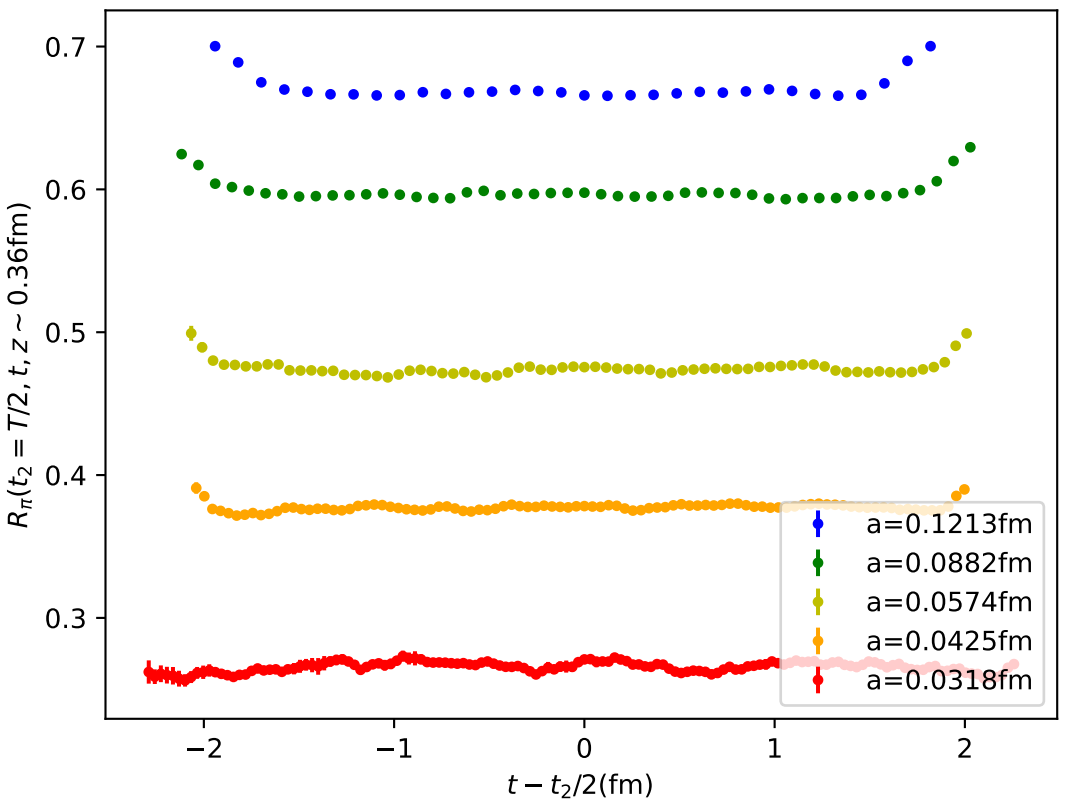
\includegraphics[width=8cm]{images/ME_pion.png}
   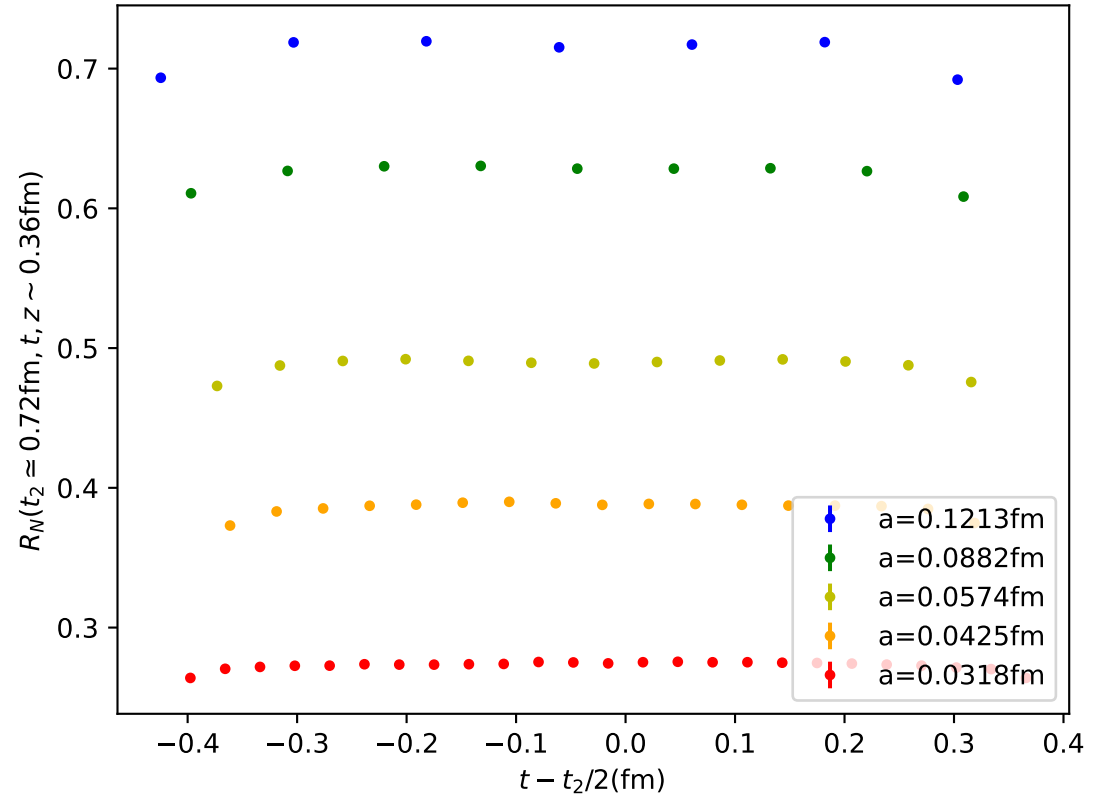
\includegraphics[width=8cm]{images/ME_nuc.png}
  \caption{$\pi$ 的裸比值 $R_{\pi}(t_2=T/2,t,z)$（上图）与核子的 $R_{N}(t_2\simeq 0.72 \textrm{fm},t,z)$（下图），取 $z\sim$ 0.36 fm。$\pi$ 情形可以看到，$t-t_2/2\in[-1,1]$ fm 区域内的数据在统计涨落范围内彼此一致；核子情形比值在 $t\sim t_2/2$ 附近同样平坦。}
  \label{fig:pion_plateau}
  \end{figure}

我们从 MILC 系综加 clover 作用量的核子与 $\pi$ 矩阵元开始。对 $\pi$ 矩阵元，我们将 $t_2=T/2$、$t\in[T/8,3T/8]$ 的 $R_{\pi}(t_2,t,z)$ 数据取平均，以获得基态矩阵元的精确估计；鉴于所用系综的 $T$ 介于 7.7 与 9.1 fm 之间，结果也理应足够精确，见图~\ref{fig:pion_plateau} 上图。注意此时 $R_{\pi}(T/2,T/4,z)$ 等于 $\langle \pi| O_{\gamma_t}(z)|\pi \rangle/2$，附加的因子 1/2 修正的是（反）周期边界条件下同时存在正向与反向传播态这一事实。核子情形噪声要大得多，尤其在大 $t_2$ 时。因此在所有情形中我们都只考虑 $t_2=2t\simeq 0.72$ fm，并把 $R_{N}(t_2,t,z)$ 绘于图~\ref{fig:pion_plateau} 下图。

 \begin{figure}[tbp]
  \centering
  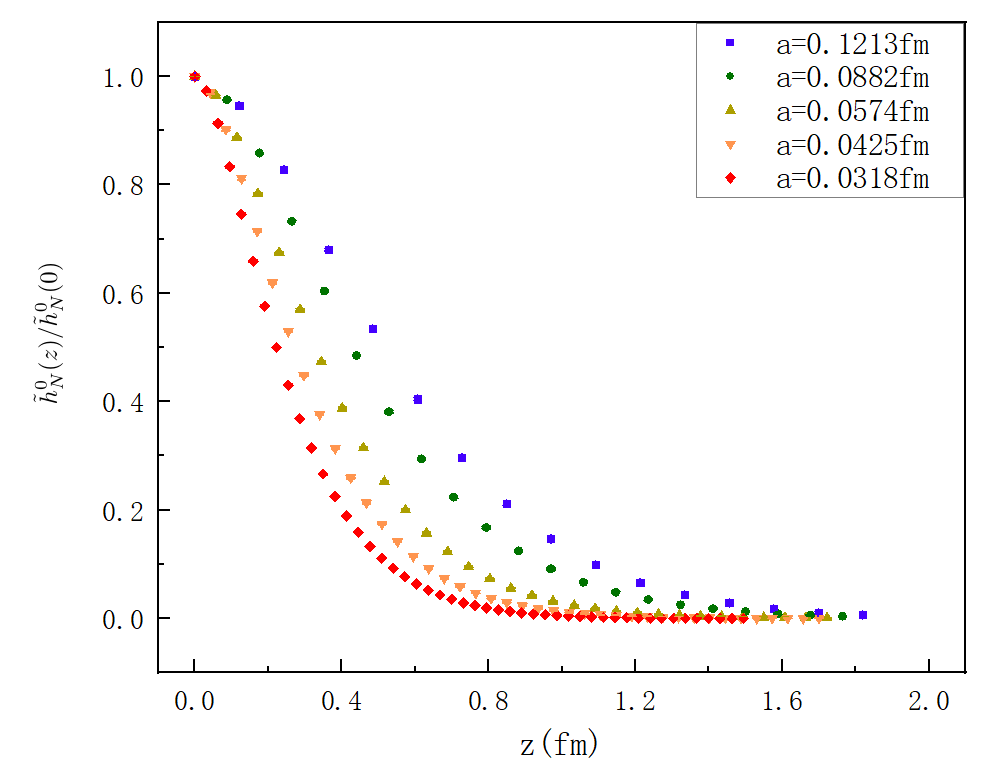
\includegraphics[width=8.5cm]{images/h_nuc_bare.png}
  \caption{静止系归一化裸核子矩阵元 $\tilde{h}^0_{N}(z)/\tilde{h}^0_{N}(0)$ 随 Wilson 链接长度 $z$ 的变化。矩阵元在大 $z$ 处快速指数衰减，且格点间距越小衰减越快。}
  \label{fig:ratio_had}
  \end{figure}

归一化的裸比值 $\tilde{h}^0_{N}(z)/\tilde{h}^0_{N}(0)$（其中 $\tilde{h}^0_{N}(z)$ 由 $t_2=2t\simeq 0.72$ fm 的 $R_{N}(t_2,t,z)$ 近似）绘于图~\ref{fig:ratio_had}，并用 jackknife 重采样施加归一化因子 $1/\tilde{h}^0_{N}(0)$，使其在所有格点间距下于 $z=0$ 处严格等于一。如图所示，线性发散使 $\tilde{h}^0_{N}(z)/\tilde{h}^0_{N}(0)$ 同时随 $z$ 与 $a$ 指数衰减，因而在 $a\to 0$ 时无法获得任何有意义的连续极限。必须进行重正化才能恢复良好的连续极限。
